% SVN info for this file
\svnidlong
{$HeadURL$}
{$LastChangedDate$}
{$LastChangedRevision$}
{$LastChangedBy$}

\chapter{Brevi cenni di Teoria degli Insiemi}
\labelAppendix{settheory}
\addtocontents{define}{\noindent\textls{\textsc{\textcolor{reddo}{Appendice B:}
\nowtitle}}
}{}
\addtocontents{theorema}{\noindent\textls{\textsc{\textcolor{reddo}{Appendice B:}
			\nowtitle}}
}{}
\begin{introduction}
‘‘La Logica è l'arte di sbagliare con confidenza.''
\begin{flushright}
	\textsc{Morris Kline,} commentando questo capitolo.
\end{flushright}
\end{introduction}
\lettrine[findent=1pt, nindent=0pt]{Q}{uando} nella vita di tutti i giorni utilizziamo i numeri naturali, lo facciamo con due scopi ben precisi:
\begin{itemize}
	\item \textbf{Contare} quanti oggetti ci sono in un insieme, associando una \textit{dimensione} ad esso: ‘‘Ci sono \textit{tre} mele nel cestino''.
	\item \textbf{Ordinare} un insieme di oggetti, ossia formare una sequenza assegnando un \textit{indice} ad ogni elemento dell'insieme: ‘‘Torino è la \textit{quarta} città italiana per numero di abitanti''.
\end{itemize}
\parshape=0
Per insiemi \textit{finiti}, non c'è apparente differenza tra i due concetti. Osserviamo che il numero di naturali (compreso lo zero) prima della $n$-esima posizione sono $n$, dunque in una sequenza di elementi indicizzata da $0$ con ultimo indice $n$ si hanno $n+1$ elementi. In altre parole, ordinando gli elementi è possibile sapere quanti sono e viceversa.\\
Questa due nozioni, come vedremo, divergono non appena generalizziamo i due concetti di ‘‘contare'' e ‘‘ordinare'' agli insiemi infiniti: ci sono molteplici ordinali infiniti che corrispondono allo stesso cardinale; inoltre, sotto certe ipotesi, potrebbero esserci insiemi che ammettono cardinalità ma che \textit{non} ammettono ordinali!\\
Lo scopo di questo capitolo aggiuntivo è cercare di dare alcune basi di \textbf{teoria degli insiemi} e \textbf{teoria degli ordini}, con il preciso scopo di spiegare come si ‘‘conta'' e si ‘‘ordina'' su insiemi infiniti.\\
Dopo una premessa sugli \textit{assiomi} sui quali baseremo i nostri ragionamenti, partiremo dal definire \textit{insiemi (ben) ordinati}, necessari per introdurre gli \textit{ordinali} (finiti e infiniti); arriveremo a parlare dell'\textit{induzione transfinita} e dell'aritmetica degli ordinali.\\
Successivamente, passeremo ai concetti di \textit{cardinalità} e \textit{numeri cardinali}, mostrando diverse proprietà (compreso lo stretto legame che li lega agli ordinali), concludendo con alcuni importanti teoremi e congetture.\\
Per maggiori approfondimenti rimandiamo a \cite{jech:2003settheory} e \cite{andretta:2021elements}.
\section{Teoria degli insiemi di Zermelo-Fraenkel e Assioma di Scelta}
Intuitivamente, un \textit{insieme} è una collezione di tutti gli elementi che soddisfano una certa proprietà. Potremmo dunque definire il seguente assioma...
\begin{falseaxiom}[Assioma della comprensione]
	Se $P$ è una proprietà, allora esiste un insieme degli elementi che soddisfano tale proprietà:
	\begin{equation*}
		Y=\left\{x \ \middle| \ P\left(x\right)\right\}
	\end{equation*}
\end{falseaxiom}
... che è però \textbf{falso} per il famoso \textbf{Paradosso di Russell}.
\begin{examplewt}[Paradosso di Russell]
	Si consideri l'insieme $S$ i cui elementi sono tutti e soli gli insiemi che non sono elementi di loro stessi:
	\begin{equation*}
		S=\left\{X \ \middle| \ X\notin X\right\}
	\end{equation*}
L'insieme $S$ appartiene a $S$? Se $S$ appartiene a $S$, allora $S$ non è un elemento di se stesso e quindi si ha $S\notin S$; d'altro canto, se $S\notin S$, allora per definizione di $S$ necessariamente $S$ appartiene a $S$. In ogni caso abbiamo un assurdo.
\end{examplewt}
Poiché $S$ non è un insieme, dobbiamo sostituire questo assioma intuitivo ma errato. Per questo si introduce una versione debole di esso, lo \textit{Schema assiomatico\footnote{Per \textbf{schema assiomatico} si intende che c'è un assioma per ogni proprietà $P$.} di Separazione}.
\begin{center}
{\small 	\emph{Se $P$ è una proprietà, allora per ogni insieme $X$ esiste un insieme degli elementi di $X$ che la soddisfano.}}
\end{center}
Osserviamo che questi assiomi \textit{non} permettono di costruire insiemi, ma solo \textit{sottoinsiemi} di altri insiemi già noti. In realtà, lo Schema assiomatico di Separazione è troppo debole per poterci costruire una teoria solo su di essi (non si può neanche definire propriamente l'unione di insiemi!), dunque abbiamo bisogno di integrare opportunamente con ulteriori assiomi.\\
Di seguito enunciamo, senza analizzarli nel dettaglio, gli assiomi di Zermelo-Fraenkel. La teoria degli insiemi basata su questi assiomi è detta, per ovvi motivi, \textbf{teoria di Zermelo-Fraenkel}\index{teoria!di Zermelo-Fraenkel} ($\mathsf{ZF}$); denotiamo con $\mathsf{ZFC}$ la teoria $\mathsf{ZF}$ con l'Assioma della Scelta ($\mathsf{AC}$).
\begin{axiom}[Assioma di Estensionalità]
	 Se $X$ e $Y$ hanno gli stessi elementi, allora $X=Y$.
\end{axiom}
\begin{axiom}[Assioma della Coppia]
	Per ogni $a$ e $b$ esiste un insieme $\{a,b\}$ che contiene esattamente $a$ e $b$.
\end{axiom}
\begin{axiom}[Schema assiomatico di Separazione]
	Se $P$ è una proprietà di parametro $p$, allora per ogni insieme $X$ e per ogni parametro $p$ esiste un insieme che contiene tutti gli elementi $u\in X$ che hanno la proprietà $P$:
	\begin{equation*}
		Y=\{u\in X\mid P\left(u,p\right)\}
	\end{equation*}
\end{axiom}
\begin{axiom}[Assioma dell'Unione]
	Per ogni insieme $X$ esiste l'insieme dato dall'unione di tutti gli elementi di $X$
	\begin{equation*}
		Y=\bigcup X
	\end{equation*}
\end{axiom}
\begin{axiom}[Assioma dell'Insieme delle Parti]
	Per ogni insieme $X$ esiste un insieme di tutti i sottoinsiemi di $X$, detto \textbf{insieme delle parti}:
	\begin{equation*}
		Y=\setpart{X}
	\end{equation*}
\end{axiom}
\begin{axiom}[Assioma dell'Infinito]
	Esiste un insieme infinito.
\end{axiom}
\begin{axiom}[Schema assiomatico di rimpiazzamento]
	Se una classe $F$ è una funzione, allora per ogni $X$ esiste un insieme \textbf{immagine}:
	\begin{equation*}
		Y=F(X)=\{F(x)\mid x\in X\}
	\end{equation*}
\end{axiom}
\begin{axiom}[Assioma di Regolarità]
	Ogni insieme non vuoto ha un minimo rispetto all'ordine dato da $\in$.
\end{axiom}
\begin{axiom}[Assioma di Scelta]
	Ogni famiglia di insiemi non vuoti ha una funzione di scelta.
\end{axiom}
\section{Relazioni d'ordine parziale e buon ordine}
\begin{define}[Relazione d'ordine parziale {(debole)} e totale]
	Una relazione binaria $\leq$ su un insieme $P$ è un \textbf{ordine parziale (debole)}\index{ordine parziale} di $P$ se è
	\begin{enumerate}
		\item \textbf{Riflessiva:} $p\leq p,\ \forall p\in P$.
		\item \textbf{Transitiva:} se $p\leq q$ e $q\leq r$, allora $p\leq r$.
	\end{enumerate}
	La coppia $\left(P,\leq\right)$ viene detta \textbf{insieme parzialmente ordinato}.\\
	Un ordine parziale è \textbf{totale}\index{ordine parziale!totale} se vale anche
	\begin{enumerate}
		\setcounter{enumi}{3}
		\item \textbf{Confrontabilità:} $p\leq q$ o $q\leq p,\ \forall p,q\in P$.
	\end{enumerate}
\end{define}
\begin{define}[Relazione d'ordine parziale  {(forte)} e totale]
	Una relazione binaria $<$ su un insieme $P$ è un \textbf{ordine parziale forte}\index{ordine parziale!forte} di $P$ se è
	\begin{enumerate}
		\item \textbf{Irriflessiva:} $p\nless p,\ \forall p\in P$.
		\item \textbf{Transitiva:} se $p<q$ e $q<r$, allora $p<r$.
	\end{enumerate}
	La coppia $\left(P,<\right)$ viene detta \textbf{insieme parzialmente ordinato}.\\
	Un ordine parziale forte è \textbf{totale} se vale anche
	\begin{enumerate}
		\setcounter{enumi}{3}
		\item \textbf{Confrontabilità:} $p<q$ o $p=q$ o $q<p,\ \forall p,q\in P$.
	\end{enumerate}
\end{define}
Abbiamo detto che i naturali, come \textit{ordinali}, servono per ordinare un insieme in una sequenza; dobbiamo capire, almeno intuitivamente, cosa intendiamo per \textit{sequenza}.\\
Una \textbf{sequenza} può essere immaginata come una lista di elementi in cui l'ordine di tali elementi è importante e la posizione di un certo elemento nella lista è determinata dalle posizioni degli elementi precedenti.\\
Pertanto, preso un generico insieme $X$, una \textbf{sequenza} deve essere una funzione da un insieme totalmente ordinato $I$, detto \textit{insieme degli indici}, che ad ogni indice $i\in I$ associa un elemento di $X$.
\begin{equation*}
	\funztot{x}{\left(I,<\right)}{X}{i}{x(i)=x_i}
\end{equation*}
\begin{center}
		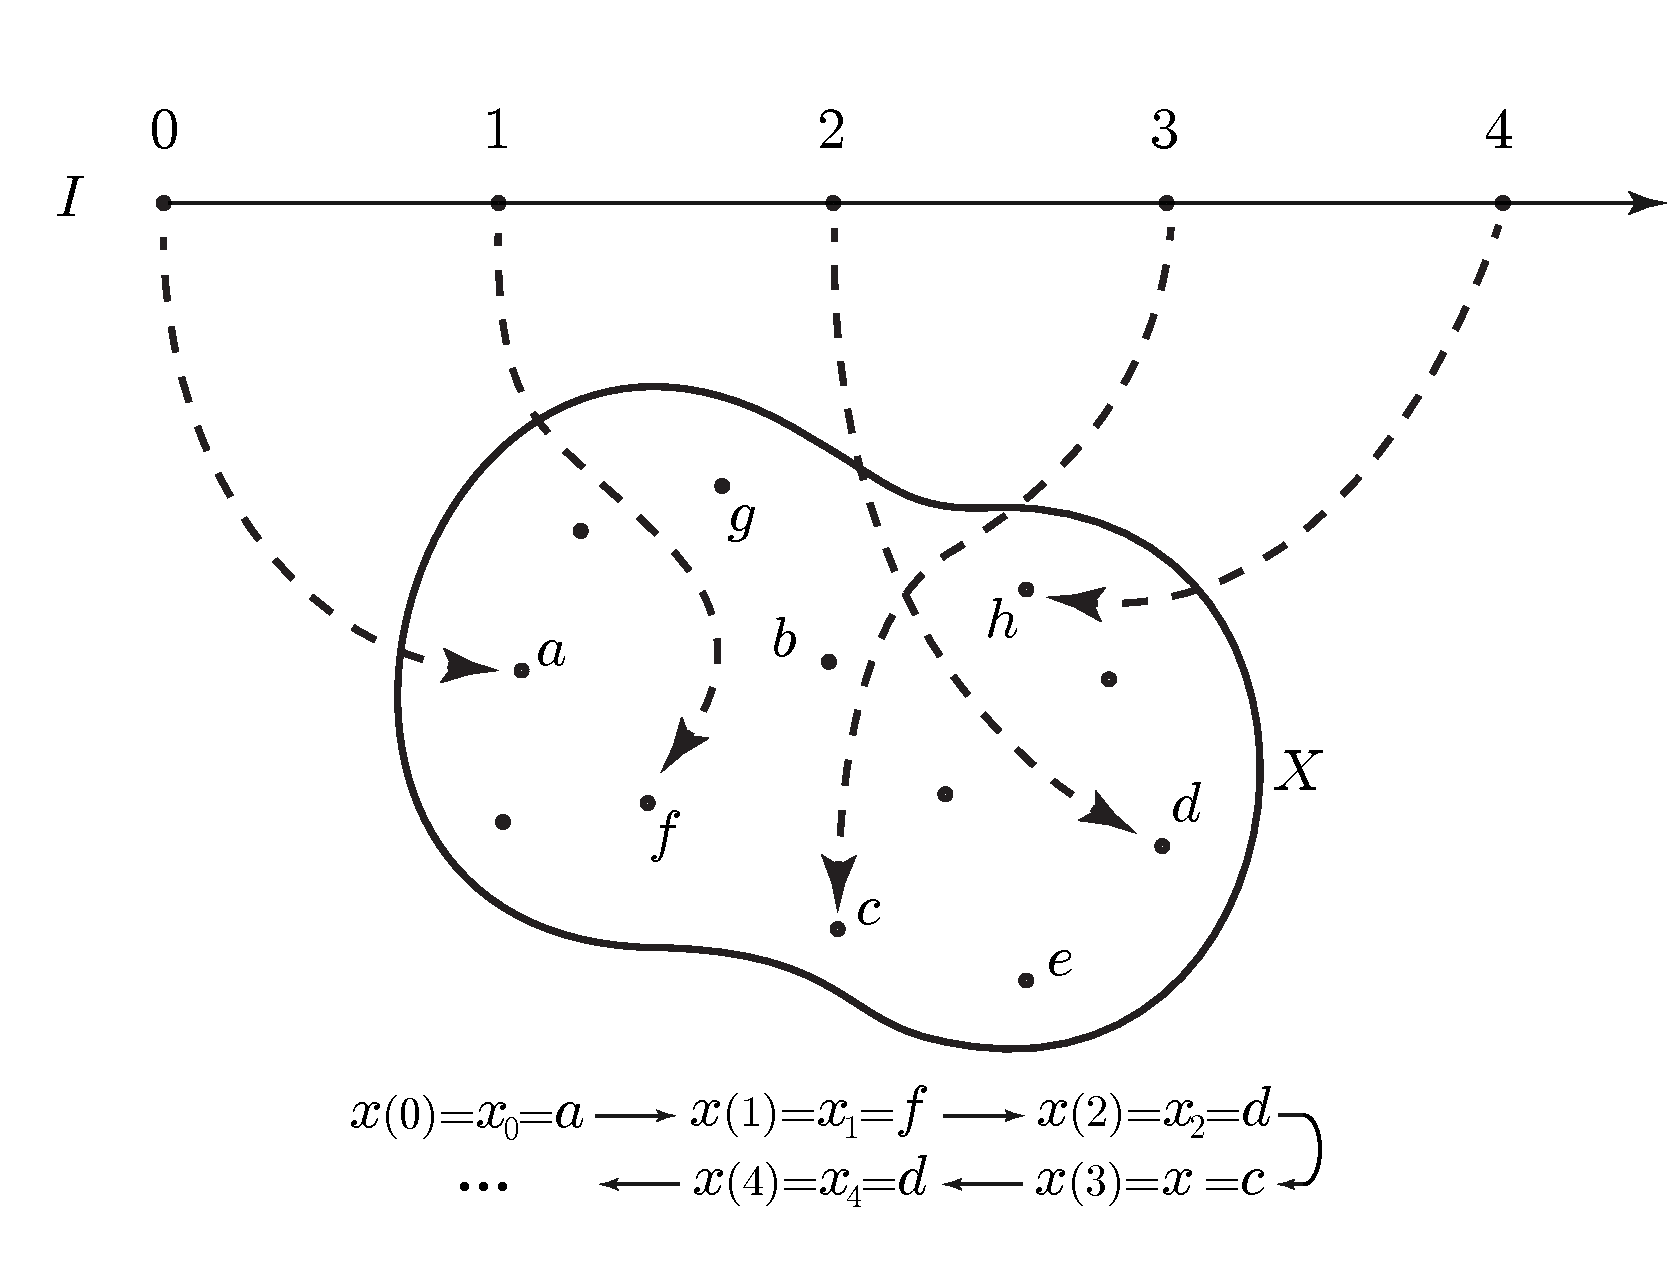
\includegraphics[trim=0cm 0cm 0cm 0cm, clip, scale=0.45]{images/settheorygrafico1.pdf}
\end{center}
È fondamentale che ci sia un \textbf{ordine} su $I$, dato che si vuole confrontare la \textit{posizione} di due elementi della sequenza: un elemento $x_i$ \textit{precede} un altro $x_j$ nella sequenza se gli indici sono tali per cui $i<j$.\\
Per soddisfare la seconda richiesta, ossia che la posizione di un certo elemento nella lista è determinata dalle posizioni degli elementi precedenti, si può pensare di definire la sequenza in modo \textit{ricorsivo}.
Tuttavia, per far ciò, \textit{non} è sufficiente che gli indici siano ordinati. Nello specifico, se $I$ contiene una \textit{sequenza infinita strettamente decrescente}, non siamo sicuri di poter definire ricorsivamente una successione a valori in $X$ indicizzata da $I$.\\
Invece, si può vedere che se $I$ \textit{non} ammette le sequenze infinite strettamente decrescenti, allora le definizioni ricorsive su $I$ sono lecite e permettono di definire univocamente una successione per ogni sequenza di indici! Dobbiamo quindi limitare quali relazioni d'ordine possiamo usare.
\begin{define}[Minimo]
	Se $\left(P,\leq\right)$ è un insieme parzialmente ordinato, $X\neq\emptyset$ un sottoinsieme di $P$ e $a\in X$, allora $a$ è \textbf{minimo}\index{minimo} di $X$ se $a\in X$ e $\forall x\in X,\ a\leq x$. Si indica $a=\min X$.
\end{define}
\begin{define}[Buon ordine]
	Un ordine parziale totale $\leq$ di $P$ è un \textbf{buon ordine} se ogni sottoinsieme $X\neq \emptyset$ di $P$ ha un minimo.
\end{define}
\begin{examples}~{}
	\begin{itemize}
		\item $\left(\naturalset,\leq\right)$ è ben ordinato.
		\item $\integerset,\ \rationalset,\ \realset$ \textit{non} sono ben ordinati rispetto all'ordine canonico $\leq$: tutti ammettono il sottoinsieme $\integerset_{<0}$ degli interi negativi, che non ha minimo.
	\end{itemize}
\end{examples}
\begin{observe}
	Ogni insieme ben ordinato \textit{non} ammette sequenze infinite strettamente decrescenti, in quanto gli elementi della sequenza formano un sottoinsieme e pertanto esso ammette minimo.
\end{observe}
\begin{intuit}
	Possiamo ora capire perché non ha particolarmente senso definire successioni indicizzate, ad esempio, rispetto a $\left(\integerset,<\right)$ o rispetto a $\left(\realset,<\right)$: non ammettendo minimo, non possiamo avere il \textit{passo base} della nostra successione definita ricorsivamente!
\end{intuit}
\begin{digression}
	Il \textbf{teorema del buon ordine}, o anche noto come \textbf{teorema di Zermelo}, afferma che \textit{ogni} insieme non vuoto può essere ben ordinato (rispetto ad un opportuno ordine).\\
	Questo teorema risulta essere vero se si considera valido l'Assioma della Scelta; in realtà, si può ulteriormente mostrare come il teorema del buon ordine risulta essere equivalente, sotto gli Assiomi di Zermelo–Fraenkel, proprio all'Assioma della Scelta!
\end{digression}
Diamo un'ultima definizione, che sarà fondamentale per collegare gli insiemi ben ordinati con gli ordinali.
\begin{define}[Funzioni monotone e isomorfismi d'ordine]
	Siano $\left(P,\leq_P\right)$ e $\left(Q,\leq_Q\right)$ due insiemi parzialmente ordinati. Una funzione $\funz{f}{P}{Q}$ è \textbf{monotona}\index{funzione!monotona} se
	\begin{equation}
		x\leq_P y\implies f(x)\leq_Q f(y)
	\end{equation}
Se una funzione monotona è biettiva e l'\textit{inversa} è monotona, allora $f$ è una \textbf{isotonia}\index{isotonia} o \textbf{isomorfismo d'ordine}.
\end{define}
\section{Ordinali}
Supponiamo di aver preso un insieme degli indici $I$ e, dopo aver posto un buon ordine su di esso, di aver definito una successione nel modo che abbiamo detto nella sezione precedente. Allora, sulla base della definizione intuitiva data nell'introduzione, gli indici scelti fungono proprio da ordinali.\\
Supponiamo ora di prendere un altro insieme di indici $J$ ben ordinati e determinare una successione sulla base di essi. Per questa nuova successione gli elementi di $J$ fanno da ordinale, ma hanno qualcosa in comune con gli indici $I$? Sono gli stessi ordinali o sono ordinali differenti? Potremmo mostrare che c'è un isomorfismo d'ordine tra $I$ e $J$: in questo modo avremmo gli stessi ordinali \textit{a meno di isomorfismo}.\\
Si mostra facilmente che, come ci si aspetterebbe da una funzione chiamata ‘‘isomorfismo'', essere isotonici è una \textbf{relazione di equivalenza} e gli insiemi parzialmente ordinati sono partizionati da essi. Da qui in poi queste classi di equivalenza le chiameremo \textbf{tipi d'ordine}\index{tipo d'ordine}.\\
Georg \textbf{Cantor} (1845 - 1918) definì un numero ordinale proprio come il tipo d'ordine di insiemi \textit{ben ordinati}. Tuttavia, l'indiscutibile appeal intuitivo che questa definizione emana ha due svantaggi:
\begin{enumerate}
	\item I tipi di ordine sono particolarmente ampi: il solo tipo associato all'ordinale $1$, di cui vedremo tra poco la definizione precisa in senso insiemistico, contiene \textbf{tutti} i singoletti, tra cui anche il singoletto $\{1\}$.
	\item In tutte le dimostrazioni che si basano sulle classi di equivalenza è necessario scegliere un rappresentante e controllare che i risultati non dipendono dalla scelta fatta.
\end{enumerate}
Fu John \textbf{von Neumann} (1903-1957)  a proporre un approccio che risolva questi problemi, ma che risulti in tutto e per tutto equivalente alla costruzione originale di Cantor: invece di vedere gli ordinali come classi di equivalenza, definire degli \textit{insiemi canonici} ben ordinati, che chiameremo \textit{ordinali}, e mostrare che ogni insieme ben ordinato è isomorfo ad uno e un solo insieme ordinale. Uno degli aspetti geniali di questa definizione è di definire gli ordinali sulla base degli ordinali che lo precedono, generalizzando ciò che succede per i numeri naturali quando usati per ordinare: un elemento è il \textit{quarto} perché segue il \textit{terzo}, che a sua volta segue il \textit{secondo}, che a sua volta segue il \textit{primo}.\\
Innanzitutto, diamo una definizione formale dei naturali come una famiglia di particolari insiemi costruiti \textit{ricorsivamente dall'insieme vuoto}.
\begin{define}[Numeri naturali]
	I \textbf{numeri naturali} $0,1,2,\ldots$ sono costruiti ricorsivamente nel seguente modo:
	\begin{equation}
		\begin{array}{l}
			0\coloneqq \emptyset\\
			n+1\coloneqq n\cup \left\{n\right\} = \left\{0,\ldots,n\right\}
		\end{array}
	\end{equation}
\end{define}
In altre parole:
\begin{equation*}
	\begin{array}{l}
		0=\left\{\emptyset\right\}\\
		1=\left\{0\right\}=\left\{\emptyset,\left\{\emptyset\right\}\right\}\\
		2=\left\{0,1\right\}=\left\{\emptyset,\left\{\emptyset\right\}, \left\{\emptyset,\left\{\emptyset\right\}\right\}\right\}\\
		\dots
	\end{array}
\end{equation*}
I naturali sono tutti degli insiemi \textit{ben ordinati} e, in particolare, sono anche \textit{transitivi}.
\begin{define}[Transitività]
	Un insieme $T$ è \textbf{transitivo}\index{transitività} se ogni elemento di $T$ è un sottoinsieme di $T$; in altre parole,
	\begin{equation}
		T\subseteq \setpart{T}
	\end{equation}
	o, equivalentemente, se $x\in T$ e $y\in x$, allora $y\in T$.
\end{define}
Possiamo generalizzare la costruzione astratta dei naturali per definire più genericamente i \textit{numeri ordinali}.
\begin{define}[Ordinale]
	Un insieme è un \textbf{ordinale}\index{ordinale} se è transitivo e ben ordinato dalla relazione d'appartenenza $\in$.\\
	Definiamo inoltre una relazione sulla classe di tutti gli ordinali $\mathrm{Ord}$:
	\begin{equation}
		\alpha<\beta\iff\alpha\in\beta
	\end{equation}
\end{define}
\begin{example}
	Per la definizione astratta di naturale, i \textbf{numeri naturali} sono tutti ordinali per definizione.
\end{example}
Dalla sola definizione seguono quasi immediatamente le seguenti proprietà.
\begin{lemmingqed}[Relazioni tra ordinali]
	Valgono le seguenti:
\begin{enumerate}
	\item Se $\alpha$ è un ordinale e $\beta\in\alpha$, allora $\beta$ è un ordinale.
	\item Se $\alpha\neq\beta$ sono ordinali e $\alpha\subsetneqq\beta$, allora $\alpha\in\beta$.
	\item Se $\alpha,\ \beta$ sono ordinali, allora si ha o $\alpha\subseteq\beta$ oppure $\beta\subseteq\alpha$.\qedhere
\end{enumerate}
\end{lemmingqed}
Da questo lemma possiamo ricavare una serie di proprietà importanti:
\begin{itemize}
	\item $<$ è una relazione d'ordine totale nella classe $\mathrm{Ord}$:
	\item Per ogni ordinale $\alpha$ si ha
	\begin{equation*}
		\alpha=\left\{\beta\in\mathrm{Ord} \ \middle| \ \beta<\alpha\right\}
	\end{equation*}
ossia un ordinale contiene \textbf{tutti} gli ordinali che lo precedono.
\item Se $C$ è una classe non vuota di ordinali, allora
\begin{equation*}
	\bigcap C=\inf C\in C
\end{equation*}
è un ordinale
\item Se $X$ è una insieme non vuoto di ordinali, allora
\begin{equation*}
	\bigcup X=\sup X
\end{equation*}
è un ordinale.
\item Per ogni $\alpha$ ordinale, $\alpha\cup\left\{\alpha\right\}$ è un ordinale ed è l'estremo inferiore di tutti gli ordinali che lo seguono.
\begin{equation*}
		\alpha\cup\{\alpha\}=\inf\{\beta\in\mathrm{Ord}\mid\beta>\alpha\}
\end{equation*}
\end{itemize}
\begin{intuit}
	La relazione $<$ indotta da $\in$ sugli ordinali si può vedere come una generalizzazione della relazione d'ordine che conosciamo bene sui naturali. Dopotutto, per essi le due relazioni coincidono!
\end{intuit}
\subsection{Ordinali successori e ordinali limiti}
Data la relazione d'ordine che caratterizzano gli ordinali e sulla base di questi fatti, ha senso definire
\begin{equation*}
	\alpha+1=\alpha\cup\{\alpha\}
\end{equation*}
il \textbf{successore}\index{successore} di $\alpha$.\\
Consideriamo ora un ordinale $\alpha$. Se esiste un ordinale $\beta$ tale per cui $\alpha=\beta+1$, si può dire che $\alpha$ è un \textbf{ordinale successore}. Non è sempre detto che però tale $\beta$ esisti! Un ordinale di questo tipo, per quanto osservato, deve essere successivo a degli ordinali, ma non deve essere il diretto successore di alcun altro ordinale. Utilizzando la terminologia dell'analisi, questo tipo di ordinale è detto \textbf{ordinale limite}\index{ordinale!limite} e
\begin{equation}
	\alpha=\sup\{\beta\in\mathrm{Ord}\mid\beta<\alpha\}=\bigcup\alpha.
\end{equation}
Si considera anche lo \textit{zero} un ordinale limite: si pone $0=\sup\emptyset$.\\
Consideriamo dunque i numeri naturali: ogni numero ha per definizione un successivo e ogni numero è successore di un altro. Segue dunque una domanda esistenziale: c'è qualcosa dopo \textit{tutti} i naturali? La risposta, in teoria degli insiemi, è sì: dopo $0$, $1$, $2$, eccetera, eccetera, si raggiunge un nuovo ordinale, che non è successore di alcun naturale ma che è successivo a tutti: $\omega$.
\begin{define}[Ordinali finiti e transfiniti]
	Si denomina con $\omega$ il più piccolo ordinale limite non zero: esso è il tipo di ordine dei naturali $\naturalset$ e si può identificare con esso.\\
	Gli ordinali prima di $\omega$, ossia i numeri naturali, sono detti ordinali \textbf{finiti}\index{ordinale!finito}, mentre $\omega$ e gli ordinali che seguono sono detti ordinali \textbf{transfiniti}\index{ordinale!transfinito} o \textit{infiniti}.
\end{define}
\begin{intuit}\label{visualizzazioneordinali}
	Come possiamo immaginare gli ordinali transfiniti successivi a $\omega$?\\
	Proviamo prima a guardare agli ordinali da nuovi punti di vista: invece che vederli ‘‘semplicemente'' come insiemi, li possiamo vedere visivamente come sequenze rispetto a $<$, in due modi: la prima è più corretta e fedele alla definizione, mentre la seconda è impropria e - secondo la definizione - errata, ma ci permette di fare alcune intuizioni utili.
	\begin{itemize}
		\item La sequenza di tutti gli ordinali che lo precedono:
		\begin{equation*}
			5\colon 0<1<2<3<4
		\end{equation*}
		\item La sequenza di tutti gli ordinali che lo precedono e l'ordinale stesso:
		\begin{equation*}
			5\colon 0<1<2<3<4\textcolor{red}{<5}
		\end{equation*}
	\end{itemize}
Se $\omega$ è identificato con $\naturalset$, allora le due visualizzazioni sono
	\begin{align*}
		\omega&\colon0<1<2<3<\ldots\\
		\omega&\colon0<1<2<3<\ldots\textcolor{red}{<\omega}
	\end{align*}
La prima visualizzazione coincide la classica rappresentazione dei naturali naturali, mentre la seconda suggerisce qualcos'altro: dopo tutti i naturali ho un elemento nuovo che tuttavia si comporta in modo estremamente simile allo \textit{zero} - dopotutto, non è successore di alcun altro numero, ma ammette un successore.\\
L'idea è quindi di \textbf{rietichettare} $\omega$ con $0'$, $\omega+1$ con $1'$ e così via. In questo modo, un ordinale come $\omega+3$ diventa 
\begin{align*}
	\omega+3&\colon0<1<2<3<\ldots<0'+1'+2'\\
	\omega+3&\colon0<1<2<3<\ldots<0'+1'+2'\textcolor{red}{+3'}
\end{align*}
Questo ragionamento permette di immaginare numeri più complessi: l'ordinale $\omega+\omega$ coincide con due copie dei naturali, la cui seconda copia segue completamente alla destra della prima:
\begin{align*}
	\omega+\omega&\colon0<1<2<3<\ldots<0'<1'<2'<3'<\ldots\\
	\omega+\omega&\colon0<1<2<3<\ldots<0'<1'<2'<3'<\ldots\textcolor{red}{<0''}
\end{align*}
\end{intuit}
Gli ordinali $\omega,\ \omega+1,\ \ldots, \omega\cdot 2,\ \ldots \omega^{\omega}\cdot $ sono tutti ordinali numerabili e riguardando l'ordinamento di insiemi infiniti detti \textit{numerabili}. L'ordinale limite che segue dopo tutti gli ordinali numerabili è indicato come $\omega_1$ ed è il primo ordinale non numerabile.\\ 
Concludiamo la sezione con una definizione che successivamente riprenderemo quando parleremo di cardinalità.
\begin{define}[Insiemi finiti e infiniti.]
	Un insieme $X$ è detto \textbf{finito}\index{insieme!finito} se c'è una biezione tra $X$ e un naturale $n\in\naturalset$, con $n$ inteso come insieme.\\
	Se $X$ non è finito è detto \textbf{infinito}\index{insieme!infinito}.
\end{define}
\subsection{Isomorfismo dell'ordinale con gli insiemi ben ordinati}
Concludiamo senza dare dimostrazione il teorema che permette di concludere la definizione di ordinale secondo von Neumann.
\begin{theoremaqed}[Isotonia tra ordinali e insiemi ben ordinati]
	Ogni insieme ben ordinato è isomorfo ad un unico ordinale.
\end{theoremaqed}
Questo è il motivo per cui si può identificare $\omega$ con $\naturalset$: l'insieme dei naturali è un insieme ben ordinato e si può mostrare l'isomorfismo d'ordine con il più piccolo ordinale limite non nullo.
\subsection{Induzione transfinita}
Ricordiamo uno dei modi per enunciare l'\textit{induzione} sui naturali. 
\begin{theoremaqed}[Induzione]
	Sia $A$ un sottoinsieme di $\naturalset$ e si supponga che
	\begin{enumerate}
		\item $0\in A$.
		\item Se $n\in A$, allora $n+1\in A$.
	\end{enumerate}
	Allora $A=\naturalset$.
\end{theoremaqed}
Con ciò che abbiamo introdotto possiamo generalizzare facilmente questa proprietà agli ordinali anche non finiti.
\begin{theorema}[Induzione transfinita]
	Sia $C$ una classe di ordinali e si supponga che
	\begin{enumerate}
		\item $0\in C$.
		\item Se $\alpha\in C$, allora $\alpha+1\in C$.
		\item Se $\alpha$ è un ordinale limite non zero e si ha $\beta\in C,\ \forall \beta<\alpha$, allora $\alpha\in C$.
	\end{enumerate}
Allora $C=\mathrm{Ord}$.
\end{theorema}
\begin{demonstration}
	Se $C=\mathrm{Ord}$ abbiamo finito. Altrimenti, sia $\alpha$ il più piccolo ordinale\footnote{Possiamo farlo in quanto un ordinale è ben ordinato.} che \textit{non} appartiene a $C$.
	\begin{itemize}
		\item Se $\alpha=0$ si ha subito l'assurdo per l'ipotesi $1$.
		\item Se $\alpha$ è un ordinale successore, allora sia $\beta$ l'ordinale tale per cui $\alpha=\beta+1$: per contronominale sulla ipotesi 2. si ha
		\begin{equation*}
			\alpha=\beta+1\notin C\implies \beta\notin C,
		\end{equation*}
		ma allora essendo $\beta<\alpha$ si ha una contraddizione perché $\alpha$ non è più il più piccolo ordinale non in $C$.
		\item Se $\alpha$ è un ordinale limite non nullo, allora per contronominale sull'ipotesi $3.$ si ha che
		\begin{equation*}
			\exists \beta<\alpha\colon\beta\notin C
		\end{equation*}
		e come prima essendo $\beta<\alpha$ si ha una contraddizione perché $\alpha$ non è più il più piccolo ordinale non in $C$.\qedhere
	\end{itemize}
\end{demonstration}
\subsection{Sequenze e limite}
Diamo ora una definizione di \textit{successione}, che abbiamo finora visto solo intuitivamente.
\begin{define}[Successione]
	Una successione è una funzione il cui dominio è un ordinale $\alpha$. La notazione canonica per una sequenza è
	\begin{equation*}
		\left<a_\xi \ \middle| \ \xi<\alpha\right>
	\end{equation*}
\end{define}
\begin{examples}~
	\begin{itemize}
		\item Una successione finita è una funzione sul dominio finito $\left\{i\in\naturalset\mid i<n\right\}$ per qualche $n\in\naturalset$. Viene anche detta anche \textbf{sequenza di lunghezza} $n$.
		\item Una successione nel senso classico del termine è una funzione su $\naturalset$ o, equivalentemente, sull'ordinale $\omega$. Si può indicare come
			\begin{equation*}
			\left<a_n \ \middle| \ n<\omega\right>
		\end{equation*}
	\end{itemize}
\end{examples}
\begin{define}[Limite di una successione]
	Sia $\alpha>0$ un ordinale limite e sia $\left<\gamma_\xi \ \middle| \ \xi<\alpha\right>$ una successione \textbf{non decrescente} di ordinali, cioè
	\begin{equation*}
		\xi <\eta \implies \gamma_\xi\leq \gamma_\eta.
	\end{equation*}
	Si definisce il \textbf{limite}\index{limite} di una successione
	\begin{equation}
		\lim_{\eta\to \alpha}\gamma_\xi=\sup\left\{\gamma_\xi\mid\xi<\alpha\right\}
	\end{equation}
\end{define}
\subsection{Aritmetica degli ordinali}
\paragraph{Addizione}
\begin{define}[Addizione di ordinali]
	Per ogni ordinale $\alpha$ si ha
	\begin{enumerate}
		\item \textbf{Zero come identità:}
		$\alpha+0=\alpha$
		\item \textbf{Associatività:}
		\begin{equation*}
			\alpha+\left(\beta+1\right)=\left(\alpha+\beta+1\right),\ \forall \beta
		\end{equation*}
		Più in generale, si ha
		\begin{equation*}
			\alpha+\left(\beta+\gamma\right)=\left(\alpha+\beta\right)+\gamma,\ \forall \beta,\ \forall\gamma
		\end{equation*}
		\item \textbf{Somma come limite:}
		\begin{equation*}
			\alpha+\beta=\lim_{\eta\to\beta}\left(\alpha+\eta\right),\ \text{per ogni ordinale limite}\ \beta>0
		\end{equation*}
	\end{enumerate}
\end{define}
\begin{attention}
	L'addizione di ordinali \textbf{non} è commutativa. Ad esempio, $1+\omega=\omega\neq\omega+1$.
\end{attention}
\begin{intuit}
	Prima di dimostrarlo formalmente, cerchiamo di capire intuitivamente perché questo non accade. Riprendendo la prima delle due visualizzazioni introdotta a pag. \pageref{visualizzazioneordinali}, scriviamo $1+\omega$ e $\omega+1$, dove etichettiamo $\omega$ con $0'$.
	\begin{align*}
		1+\omega&\colon0<0'<1'<2'<3'<\ldots\\
		\omega+1&\colon0<1<2<3<\ldots<0'
	\end{align*}
	Notiamo che nel primo caso $0'$ (cioè $\omega$) ha un predecessore, $0$, cosa che normalmente \textit{non} ha; rinominando $n'$ con $n+1$ otteniamo che la sequenza assomiglia in realtà a $\omega$ stesso, cioè possiamo dire che $1+\omega=\omega$. D'altro canto, $\omega+1$ ha un elemento massimo, che è $0'$, mentre $\omega$ non lo ha!
\end{intuit}
\begin{examplewt}[Non commutatività dell'addizione di ordinali]
	Mostriamo che
	\begin{equation*}
		1+\omega=\omega\neq\omega+1
	\end{equation*}
 	Infatti, il termine di sinistra diventa
 	\begin{align*}
 		1+\omega&=\lim_{\eta\to \omega}\left(1+\xi\right)=\sup\left\{1+\xi \ \middle| \ \xi<\omega\right\}=\bigcup_{\xi<\omega}\left\{1+\xi\right\}=\\
 		&=1\cup 2\cup 3\cup \ldots=\{0\}\cup\{0,1\}\cup\{0,1,2\}\cup\ldots\naturalset=\omega
 	\end{align*}
 	e per definizione $\omega<\omega+1$ e dunque sono due ordinali distinti.
\end{examplewt}
In realtà è molto raro che $\alpha+\beta$ sia uguale a $\beta+\alpha$: ciò succede se e solo se $\alpha=\gamma \cdot m$ e $\beta=\gamma \cdot n$ con $\gamma$ ordinale e $m,\ n$ naturali e $\cdot$ la moltiplicazione tra ordinali che vedremo tra poco.
\paragraph{Moltiplicazione}
\begin{define}[Moltiplicazione di ordinali]
	Per ogni ordinale $\alpha$ si ha
	\begin{enumerate}
		\item \textbf{Zero come elemento nullo:}
		$\alpha\cdot0=0$
		\item \textbf{Distributiva da sinistra:}
		\begin{equation*}
			\alpha\cdot\left(\beta+1\right)=\alpha\cdot\beta+\alpha,\ \forall \beta
		\end{equation*}
		\item \textbf{Associativa:}
		\begin{equation*}
			\alpha\cdot\left(\beta\cdot\gamma\right)=\left(\alpha\cdot\beta\right)\cdot\gamma,\ \forall \beta,\ \gamma
		\end{equation*}
		\item \textbf{Prodotto come limite:}
		\begin{equation*}
			\alpha\cdot\beta=\lim_{\eta\to\beta}\left(\alpha\cdot\eta\right),\ \text{per ogni ordinale limite}\ \beta>0
		\end{equation*}
	\end{enumerate}
\end{define}
\begin{attention}
	La moltiplicazione di ordinali \textbf{non} è commutativa e neanche distributiva da destra. Ad esempio, $\left(1+1\right)\cdot\omega=\omega\neq\omega\cdot\left(1+1\right)=\omega+\omega$.
\end{attention}
\begin{examplewt}[Non commutatività della moltiplicazione di ordinali]
	Mostriamo che
	\begin{equation*}
		\left(1+1\right)\cdot\omega=2\omega=\omega\neq\omega\cdot\left(1+1\right)=\omega\cdot 2=\omega+\omega
	\end{equation*}
	Infatti, il termine di sinistra diventa
	\begin{align*}
		\left(1+1\right)\cdot\omega&=2\cdot\omega=\lim_{\eta\to \omega}\left(2\cdot\xi\right)=\sup\left\{2\cdot\xi \ \middle| \ \xi<\omega\right\}=\bigcup_{\xi<\omega}\left\{2\cdot\xi\right\}=\\
		&=2\cdot 0\cup2\cdot 1\cup 2\cdot2\cup 2\cdot3\cup \ldots=0\cup 2\cup 6\cup\ldots=\\
		&=\emptyset\cup\{0,1\}\cup\{0,1,2,3,4,5\}\cup\ldots=\naturalset=\omega
	\end{align*}
	e per definizione $\omega<\omega+\omega$ e dunque sono due ordinali distinti.
\end{examplewt}
\paragraph{Esponenziazione}
\begin{define}[Esponenziazione di ordinali]
		Per ogni ordinale $\alpha$ si ha
	\begin{enumerate}
		\item \textbf{Esponenziazione per zero:}
		$\alpha^0=1$
		\item \textbf{Distributiva dell'esponenziale rispetto all'esponente:}
		\begin{equation*}
			\alpha^{\beta+1}=\alpha^\beta\cdot\alpha,\ \forall \beta
		\end{equation*}
		\item \textbf{Prodotto come limite:}
		\begin{equation*}
			\alpha^{\beta}=\lim_{\eta\to\beta}\left(\alpha^\eta\right),\ \text{per ogni ordinale limite}\ \beta>0
		\end{equation*}
	\end{enumerate}
\end{define}
\paragraph{Aritmetica degli ordinali e aritmetica degli interi}
Abbiamo visto che le operazioni con i numeri ordinali hanno notevoli differenze da queste 
\begin{property}[Aritmetica degli ordinali e aritmetica degli interi]
	Valgono le seguenti proprietà:
	\begin{enumerate}
		\item Se $\beta<\gamma$, allora
		\begin{equation*}
			\alpha+\beta<\alpha+\gamma,\ \forall \alpha.
		\end{equation*}
		\item Se $\alpha<\beta$, allora esiste un unico $\delta$ tale che \begin{equation*}
			\alpha+\delta=\beta.
		\end{equation*}
		\item Se $\beta<\gamma$, allora
		\begin{equation*}
			\alpha\cdot \beta<\alpha\cdot\gamma,\ \forall \alpha>0.
		\end{equation*}
		\item Se $\alpha>0$ e $\gamma$ è un ordinale arbitrario, allora esiste un unico $\beta$ e un unico $\rho<\alpha$ tale che
		\begin{equation*}
			\gamma=\alpha\cdot\beta+\rho.
		\end{equation*}
		\item Se $\beta<\gamma$ e $\alpha>1$, allora
		\begin{equation*}
			\alpha^{\beta}<\alpha^{\gamma}.\qedhere
		\end{equation*}
	\end{enumerate}
\end{property}
\begin{theoremaqed}[Teorema della forma normale di Cantor]
	Ogni ordinale $\alpha>0$ può essere rappresentato unicamente nella forma
	\begin{equation}
		\alpha=\sum_{i=1}^{+\infty}\omega^{\beta_i}\cdot k_i=\omega^{\beta_1}\cdot k_1+\cdot+\omega^{\beta_n}\cdot k_n
	\end{equation}
dove $n\geq 1,\ \alpha\geq \beta_1>\ldots>\beta_n$ e $k_1,\ \ldots, k_n$ sono naturali non nulli.
\end{theoremaqed}
Dal teorema della forma normale è possibile che ci siano degli ordinali $\alpha$ tali che
\begin{equation*}
	\alpha=\omega^{\alpha}
\end{equation*}
Il più piccolo di questi ordinali è indicato con $\epsilon_0$.
\section{Cardinalità}
\begin{comment}

\end{comment}
\begin{define}[Cardinalità]
	Due insiemi $X$ e $Y$ sono \textbf{equipotenti}\index{equipotenza} o \textbf{equinumerosi}\index{equinumerosità}, in simboli
	\begin{equation}
		X\asymp Y
	\end{equation}
	se esiste una corrispondenza \textit{biunivoca} tra i due insiemi.\\
	L'equipotenza è una \textit{relazione di equivalenza} sulle classi di tutti gli insiemi; diciamo che due insiemi $X$ e $Y$ equipotenti hanno la stessa \textbf{cardinalità}\index{cardinalità} e lo indichiamo con
	\begin{equation}
		\abs{X}=\abs{Y}
	\end{equation}
\end{define}

\subsection{Ordine delle cardinalità}
\begin{define}[Iniezione]
	Un insieme $X$ si \textbf{inietta in} $Y$, in simboli 
	\begin{equation}
		X\precsim Y
	\end{equation}
	se esiste una funzione iniettiva $\funz{f}{X}{Y}$; in tal caso scriveremo
	\begin{equation}
		\abs{X}\leq\abs{Y}
	\end{equation}
\end{define}
\begin{corollary}[Inclusione e cardinalità]\label{cardinalitàinclusione}
	Se $X\subseteq Y$, allora $X\precsim Y$ (o in termini di cardinalità, $\abs{X}\leq\abs{Y}$).
\end{corollary}
\begin{demonstration}
	Dire che $X\subseteq Y$ implica l'esistenza dell'inclusione $\incl{\iota}{X}{Y}$, la quale è per definizione una funzione iniettiva.
\end{demonstration}
\begin{attention}\label{cardinalitàugualenonimplicauguaglianzainsiemistica}
	Anche se un sottoinsieme ha la stessa cardinalità dell'insieme a cui appartiene, non è detto che siano uguali; come controesempio basta considerare i numeri naturali $\naturalset$ e numeri pari $2\naturalset$: fra i due c'è una biezione $\funz{\ }{\naturalset}{2\naturalset}$ data da $f(n)=2n$, ma i naturali contengono anche i dispari.\\
	Si può invece affermare che un sottoinsieme \textbf{finito} equipotente all'insieme a cui appartiene deve coincidere con esso.
\end{attention}
La relazione $\precsim$ (o $\leq$ se ci riferiamo alle cardinalità) è una relazione d'\textit{ordine totale}: la relazione riflessiva e transitiva sono immediate, mentre l'antisimmetrica è garantita dal seguente teorema.
\begin{theoremaqed}[Teorema di Cantor-Bernstein-Schröder]
	Se $\abs{X}\leq\abs{Y}$ e $\abs{Y}\leq\abs{X}$, allora $\abs{X}=\abs{Y}$.\\
	Equivalentemente, se esistono due funzioni \textit{iniettive}
	\begin{equation*}
		\funz{f}{X}{Y}\text{ e }\funz{g}{Y}{X}
	\end{equation*}
	allora esiste una funzione \textit{biettiva} $\funz{h}{X}{Y}$.
\end{theoremaqed}
Un'altra conseguenza importante di questo teorema è quella di poter determinare la cardinalità sulla base di sole funzioni \textit{iniettive}.
\begin{examplewt}[Un'applicazione del teorema di Cantor-Bernstein-Schröder]
	L'intervallo $\left[0,1\right]$ ha la cardinalità del continuo; infatti, possiamo considerare le seguenti funzioni iniettive:
	\begin{itemize}
		\item $\incl{\iota}{\left[0,1\right]}{\realset}$ inclusione.
		\item $\funztot{f}{\realset}{\left[0,1\right]}{x}{\frac{2\left(\arctan(x)+\frac{\pi}{2}\right)}{\pi}}$
	\end{itemize}
\end{examplewt}
La seguente proposizione permette invece stabilire una relazione di cardinalità tra dominio e codominio di una funzione \textit{suriettiva}.
\begin{proposition}[La cardinalità del dominio di una funzione suriettiva è maggiore o uguale della cardinalità del codominio]\label{cardinalitàsuriettiva}
	Sia $\surr{g}{Y}{X}$ suriettiva, con $\left(Y,\unlhd\right)$ un insieme ben ordinato. Allora esiste una funzione iniettiva $\funz{f}{X}{Y}$ tale che $g\circ f=id_X$. In altre parole,
	\begin{equation}
		\surr{g}{\left(Y,\unlhd\right)}{X}\implies X\precsim Y \left( \iff \abs{X}\leq\abs{Y}\right).\qedhere
	\end{equation}
\end{proposition}
\begin{demonstration}
	Si definisce $f$ in modo che $f(x)$ è il minimo y$\in Y$, rispetto a $\unlhd$, per cui $g\left(y\right)=x$.
\end{demonstration}
\begin{attention}
	È fondamentale l'ipotesi del buon ordine su $Y$: per insiemi non ben ordinati, la proprietà non si verifica perché non si potrebbe scegliere a priori un elemento da fissare. Tuttavia, se si assume l'Assioma della Scelta come vero allora questa proprietà è verificata per ogni insieme.
\end{attention}
\begin{example}
	Come visto\footnote{Si veda \refChapterOnly{teoriamisura}, pag. \pageref{insiemecantor}.}, dato l'insieme di Cantor $C$ si può definire una funzione $\surr{f}{C}{\left[0,1\right]}$ \textit{suriettiva}; in questo modo, $\abs{C}\geq \left[0,1\right]$ ma, in quanto $C\subseteq \left[0,1\right]$ si ha 
	\begin{equation*}
		\abs{C}=\left|\left[0,1\right]\right|
	\end{equation*}
Questa è anche una conseguenza del teorema di Cantor–Bernstein–Schröder, dato che abbiamo definito (implicitamente o esplicitamente) due funzioni iniettive $\funz{\ }{X}{Y}$ e $\funz{\ }{Y}{X}$.
\end{example}
Ci interessa anche definire una relazione d'\textit{ordine parziale forte} sulla base dell'iniezione precedentemente definita. 
\begin{define}[Iniezione stretta]
	Un insieme $X$ si \textbf{inietta strettamente in} $Y$, in simboli 
	\begin{equation}
		X\precnsim Y
	\end{equation}
	se esiste una funzione iniettiva $\funz{f}{X}{Y}$ ma non esistono funzioni suriettive $\funz{f}{X}{Y}$; in tal caso scriveremo
	\begin{equation}
		\abs{X}<\abs{Y}
	\end{equation}
\end{define}
\begin{observe}
	Si può vedere che
	\begin{equation}
		X \precnsim Y\iff X\precsim Y\wedge X\cancel\asymp Y
	\end{equation}
	o, in termini di cardinalità,
	\begin{equation}
		\abs{X}<\abs{Y}\iff \abs{X}\leq \abs{Y}\wedge \abs{X}\neq\abs{Y}
	\end{equation}
\end{observe}
\subsection{Aritmetica dei cardinali}
Possiamo definire delle \textit{operazioni aritmetiche} con i cardinali; dati $\abs{X}=\kappa$ e $\abs{Y}=\lambda$, si ha
\begin{align}
	\kappa+\lambda&=\abs{X\cup Y} \text{ se }X\text{ e }Y\text{ disgiunti}\\
	\kappa\cdot\lambda&=\abs{X\times Y}\\
	\kappa^{\lambda}&=\abs{X^Y}
\end{align}
dove con $X^Y$ indichiamo l'\textit{insieme delle funzioni} da $Y$ in $X$.\\
Queste operazioni sono ben definite se sono indipendenti dalla scelta di $X$ e $Y$.
\begin{property}[Proprietà dell'aritmetica dei cardinali]
	Valgono le seguenti proprietà:
	\begin{enumerate}
		\item L'addizione $+$ e la moltiplicazione $\cdot$ sono associative, commutative e distributive.
		\item \textbf{Distributività dell'esponenziale rispetto alla base:}
		\begin{equation}
			\left(\kappa\cdot\lambda\right)^{\mu}=\kappa^{\mu}\cdot\lambda^{\mu}
		\end{equation}
		\item \textbf{Distributività dell'esponenziale rispetto all'esponente:}
		\begin{equation}
			\kappa^{\lambda+\mu}=\kappa^{\lambda}\cdot\kappa^{\mu}
		\end{equation}
		\item \textbf{Esponenziale di un esponenziale:}
		\begin{equation}
			\left(\kappa^{\lambda}\right)^{\mu}=\kappa^{\lambda\cdot\mu}
		\end{equation}
		\item Se $\lambda\leq \mu$, allora
		\begin{equation}
			\kappa^{\mu}\leq \lambda^{\mu}
		\end{equation}
		\item Se $0<\lambda\leq \mu$, allora
		\begin{equation}
			\kappa^{\lambda}\leq \kappa^{\mu}
		\end{equation}
		\item Se $\kappa>0$, allora
		\begin{equation}
			\kappa^0=1\qquad 1^{\kappa}=1\qquad 0^\kappa=0
		\end{equation}
	\end{enumerate}
\end{property}
\subsection{Cardinalità dell'insieme delle parti}
Finché operiamo con insiemi finiti, è chiara la differenza tra le dimensioni di due insiemi; la questione è differente se si parla di insiemi infiniti: non sempre è immediata la cardinalità. Ad esempio, i numeri pari e i naturali hanno la stessa cardinalità (basta considerare $f(n)=2n$) come biezione, ma i naturali sembrano molto più grandi.\\
Si potrebbe pensare che tutti gli insiemi infiniti hanno la stessa cardinalità. Il seguente teorema ci mostra come questo \textit{non} sia il caso, e la cardinalità è un aspetto fondamentale dello studio degli insiemi infiniti.
\begin{theorema}[Teorema di Cantor]
	Per ogni insieme $X$ si ha
	\begin{equation}
		X\precnsim\setpart{X}
	\end{equation}
	\begin{equation}
		\abs{X}<\abs{\setpart{X}}
	\end{equation}
\end{theorema}
\begin{demonstration}
	Sia per assurdo $\funz{f}{X}{\setpart{X}}$ una funzione suriettiva e sia
	\begin{equation*}
		Y=\left\{x\in X\mid x\notin f(x)\right\}
	\end{equation*}
	Per la suriettività di $f$, $\exists z\in X$ tale che $f\left(z\right)=Y$; tuttavia, si ha $z\in Y\iff z\notin f\left(z\right)=Y$, il che è assurdo. Segue che $X\nasymp\setpart{X}$.\\
	Invece, la funzione
	\begin{equation*}
		\funztot{f}{X}{\setpart{X}}{x}{\left\{x\right\}}
	\end{equation*}
	è iniettiva e quindi $X\precsim\setpart{X}$. Concludendo, $X\precnsim\setpart{X}$.
\end{demonstration}
\begin{theoremaqed}[Biezione tra {$\setpart{X}$} e insieme delle funzioni da {$X$} in {$\{0,1\}$}]\label{cardinalitàsetpart}
	Dato un qualunque insieme $X$, sia $\setpart{X}$ l'insieme delle parti di $X$ e sia $2^X\coloneqq\left\{0,1\right\}^X$ l'insieme di tutte le funzioni $\funz{\ }{X}{\left\{0,1\right\}}$. Allora esiste una biezione tra $\setpart{X}$ e $2^X$, data da
	\begin{equation}
		\funztot{\Phi}{\setpart{X}}{2^X}{X}{\chi_X}
	\end{equation}
	con $\chi_X$ la \textit{funzione indicatrice} su $X$; l'inversa di tale funzione è la seguente:
	\begin{equation}
		\funztot{\Phi^{-1}}{2^X}{\setpart{X}}{f}{\left\{x\in\ X\mid f(x)=1\right\}}\qedhere
	\end{equation}
\end{theoremaqed}
\begin{demonstration}
	Per il teorema precedente, si ha una biezione tra $\setpart{X}$ e $2^{\abs{X}}\coloneqq\left\{0,1\right\}^{X}$, dunque hanno la stessa cardinalità. Per esponenziazione dei cardinali, si ha
	\begin{equation*}
		\abs{\setpart{X}}=\left|\left\{0,1\right\}^{X}\right|=\left|\left\{0,1\right\}\right|^{\abs{X}}=2^{\abs{X}}\qedhere
	\end{equation*}
\end{demonstration}
\begin{corollary}[Cardinalità dell'insieme delle parti]\label{insiemiparti}
	Se un insieme $X$ ha cardinalità $\abs{X}$, l'insieme delle parti ha cardinalità
	\begin{equation}
		\abs{\setpart{X}}=2^{\abs{X}}
	\end{equation}
\end{corollary}
Il teorema di Cantor si può quindi riformulare come segue
\begin{theoremaqed}[Teorema di Cantor, riformulato]
	Per ogni cardinale $\kappa$ si ha $\kappa<2^{\kappa}$.
\end{theoremaqed}
\subsection{Ordinali e cardinali}
Sappiamo che gli ordinali, per definizione di von Neumann, sono degli insiemi. Possiamo dare una definizione di \textit{numero cardinale} partendo proprio dal concetto di ordinale.
\begin{define}[Cardinale]
	Un ordinale $\alpha$ è detto un \textbf{cardinale}\index{cardinale} se
	\begin{equation}
		\abs{\alpha}\neq\abs{\beta},\ \forall \beta<\alpha
	\end{equation}
\end{define}
Se $W$ è un insieme ben ordinato, sappiamo che esso ha un tipo d'ordine e dunque almeno un ordinale ad esso associato. Allora consideriamo, dato $W$, il suo numero cardinale come
\begin{equation*}
	\abs{W}=\min\{\alpha\in\mathrm{Ord}\mid\abs{W}=\abs{\alpha}\}
\end{equation*}
Ricordiamo che $X$ è \textit{finito} se è in corrispondenza biunivoca con un \textit{ordinale finito} $n\in\naturalset$:
\begin{equation*}
	\abs{X}=\abs{n}
\end{equation*}
Poichè $\abs{n}=\abs{m}\iff n=m$, gli \textit{ordinali finiti} corrispondono ai \textit{cardinali finiti} e quindi $\abs{n}=n$, ossia
\begin{equation*}
	\abs{X}=n
\end{equation*}
L'ordinale $\omega$ è il più piccolo numero cardinale infinito. 
\begin{observe}
	Tutti i cardinali infiniti sono ordinali limiti.
\end{observe}
Gli ordinali infiniti che sono anche cardinali sono chiamati \textbf{aleph}\index{aleph}.
\begin{lemming}[Successori dei cardinali]
	Si può mostrare che per ogni cardinale $\alpha$ c'è un cardinale più grande di esso. Il più piccolo tra quelli più grandi di $\alpha$ viene indicato con $\alpha^{+}$ ed è detto il \textbf{cardinale successore}\index{cardinale!successore}.
\end{lemming}
In particolare, consegue anche che se $X$ è un insieme di cardinali $\sup X$ è un cardinale.\\
Definiamo allora l'enumerazione degli aleph. Indichiamo normalmente $\aleph_{\alpha}$ per i numeri cardinali e $\omega_\alpha$ per il tipo di ordine.
\begin{align*}
	\aleph_0&=\omega_0=\omega\\
	\aleph_{\alpha+1}&=\alpha_{\alpha}^{+}=\omega_{\alpha+1}\\
	\aleph_{\alpha}&=\omega_{\alpha}=\sup\left\{\omega_\beta\mid \beta<\alpha\right\}\quad\text{se}\ \alpha\ \text{è un ordinale limite}
\end{align*}
In questo modo, affermiamo che
\begin{equation}
	\abs{\naturalset}=\aleph_0
\end{equation}
Inoltre, poiché si può mostrare che $\integerset$ e $\rationalset$ sono in biezione con i naturali, anche loro hanno cardinalità $\aleph_0$.
\begin{observe}
	Dalla definizione si nota un fatto fondamentale: ci possono essere più ordinali per uno stesso cardinale. Come mai?\\
	Gli ordinali descrivono in che maniera (a meno di rietichettare i miei elementi) posso ordinare un insieme, mentre i cardinali sono una misura della dimensione di tale insieme.\\ Finché ci limitiamo ai naturali, come ben sappiamo, non c'è differenza tra ordinale e cardinale. Anzi! Ad ogni numero naturale associamo un solo ordinale e un solo cardinale - ad esempio, se devo ordinare l'insieme $\{1,2,3,4\}$ - che ha cardinalità $4$ - non importa se metto prima il 2 dell'1 o il 3 dopo il 4, dato che rinominando gli elementi ottengo sempre l'ordine canonico $0<1<2<3$.\\
	Caso differente è per gli insiemi infiniti. Ad esempio, sui naturali posso avere l'ordinamento canonico $\omega$, ma posso anche riordinarli mettendo prima tutti i naturali dispari seguiti da tutti i naturali pari:
	\begin{equation*}
		1<3<5<7<9<\ldots<2<4<6<8<10<\ldots
	\end{equation*}
	Questo ordinamento quale ha tipo d'ordine $\omega\cdot 2\neq \omega$. Tuttavia, entrambi sono ordinamenti dei naturali e quindi hanno cardinalità $\aleph_0$.
\end{observe}
La somma e il prodotto di aleph è abbastanza triviale, dato che si può mostrare che:
\begin{equation*}
	\aleph_{\alpha}+\aleph_{\beta}=\aleph_{\alpha}\cdot\aleph_{\beta}=\max\{\aleph_{\alpha},\aleph_{\beta}\}
\end{equation*}
\subsection{Cardinalità del continuo}
Abbiamo definito i cardinali per insiemi \textit{ben ordinati}, basandoci sugli ordinali. In realtà, se supponiamo l'\textit{Assioma di Scelta}, allora \textit{ogni insieme} è ben ordinato e quindi possiamo parlare di cardinali in generale in $\mathsf{ZFC}$, anche per insiemi come i \textit{reali}.
\begin{theoremaqed}[Cantor]
L'insieme dei numeri reali non è numerabile, ossia è un insieme infinito che non è in corrispondenza biunivoca con i naturali.
\end{theoremaqed}
Indichiamo con $\mathfrak{c}$ la \textbf{cardinalità dei reali} o \textbf{cardinalità del continuo}\index{cardinalità!del continuo}:
\begin{equation}
	\abs{\realset}=\mathfrak{c}
\end{equation}
Che valore ha questa cardinalità?\\
Poiché siamo in grado di calcolare la cardinalità dell'insieme delle parti di insiemi per il corollario \ref{insiemiparti}, si ha che $\abs{\setpart{\naturalset}}=2^{\aleph_{0}}$.\\
Dato che ogni numero reale è l'estremo superiore di un'opportuna sequenza di razionali minori di essa, cioè
\begin{equation*}
	r=\sup\{q\in\rationalset\mid q<r\},
\end{equation*}
si ha che la cardinalità dei reali deve essere minore dell'insieme delle sequenze in $\rationalset$, che ha cardinalità pari all'insieme delle parti di $\rationalset$, ovvero
\begin{equation*}
	\mathfrak{c}\leq\abs{\setpart{\rationalset}}=2^{\aleph_0}
\end{equation*}
D'altro canto, l'insieme di Cantor\footnote{Si veda \refChapterOnly{teoriamisura}, pag. \pageref{insiemecantor}.} si vede che è in corrispondenza diretta con tutte le sequenze di $0$ e $2$ e la cardinalità coincide con quella di $2^{\aleph_0}$. Poiché Cantor è un sottoinsieme dei reali, si ha
\begin{equation*}
	\mathfrak{c}\geq \abs{C}=2^{\aleph_0}
\end{equation*}
e quindi si può concludere per Cantor-Bernstein-Schröder che
\begin{equation*}
	\mathfrak{c}=2^{\aleph_0}
\end{equation*}
Una peculiarità di questo cardinale è che nella teoria $\mathsf{ZFC}$ \textit{non} è chiaro dove si posizioni nella gerarchia degli $\aleph$, ma Cantor formulò una congettura a riguardo: non ci sono insiemi la cui cardinalità è compresa tra quella degli interi e quella dei reali; in altre parole,
\begin{equation}
	(\mathsf{CH})\quad 2^{\aleph_0}=\aleph_1
\end{equation}
L'\textbf{ipotesi del continuo} ($\mathsf{CH}$) non può essere provata o confutata nel sistema di $\mathsf{ZFC}$.\\
Cos'è, invece, la cardinalità dell'insieme delle parti dei reali?\label{cardinalitàsetpartreali}
\begin{equation*}
\abs{\setpart{\realset}}=2^{\mathfrak{c}}
\end{equation*}
Sappiamo che è un numero \textit{ancora più grande} della cardinalità del continuo, ma non è per nulla facile capire cos'è. \\
Dato che ciò esenta gli scopi che ci siamo prefissi per questa appendice - che già di per sé è un esteso (e non necessario) approfondimento di teoria degli insiemi\footnote{Nel caso avessimo sbagliato in qualche punto, qualche logico ci illumini per favore. Io manco ho seguito \textsc{Logica}.} scritto per spiegare qualche termine usato nel capitolo di Teoria della Misura - lasciamo ad un eventuale lettore curioso qualche spunto a riguardo:
\begin{itemize}
	\item \textbf{Beth number}\\ \textcolor{redill}{\url{https://en.wikipedia.org/wiki/Beth_number}}
	\item \textbf{What is known about the power set of the real number line?}\\ \textcolor{redill}{\url{https://math.stackexchange.com/a/94000/875294}}
\end{itemize}